\section{Versuchsaufbau und -durchführung}

\subsection{Versuchsaufbau}

Der allgemeine Versuchsaufbau ist in Abbildung \ref{fig:aufbau_warmepumpe} dargestellt.


\begin{figure}
\centering
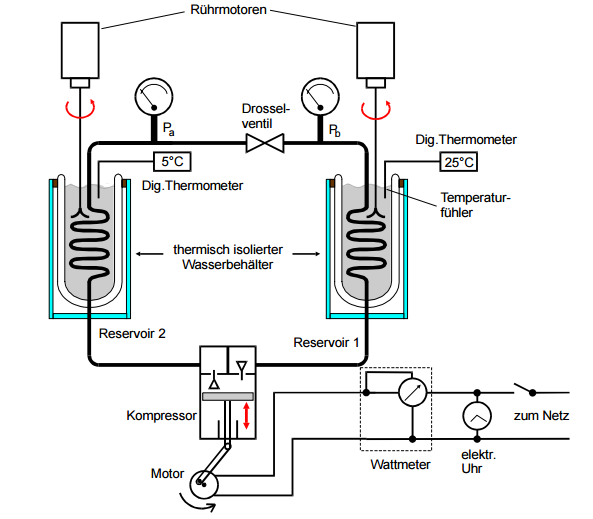
\includegraphics[width=0.9\textwidth]{bilder/versuchsaufbau_1.png}
\caption{Schematischer Aufbau einer Wärmepumpe}
\label{fig:aufbau_warmepumpe}
\end{figure}


An diesem soll auf die Funktionsweise einer Wärmepumpe erklärt werden.

In den Leitung der Wärmepumpe befindet sich ein Gas (Dichlodifluormethan) 
dieses sieht als Transportmedium.
Beginnen wir bei unserer Betrachtung, bei Reservoir $1$.
In diesem wird die Temperatur $T_1$ gemessen, während der Druck $p_b$ wirkt.
Das Gas erreicht im gasförmigen Reservoir $1$. Zu diesem Zeipunkt ist es
stark erwärmt und so unter Druck kompremiert, dass es sich im Reservoir $1$ wieder verflüssigt.
Während dessen gibt es pro Gramm Gas die Kondensationswärme $L$ and das Reservoir ab.
Dadurch wird dieses aufgeheizt.


